\subsection{Self-interpretable} 
In self-interpretable methods, the explainable procedure is intrinsic to the model. Such methods derive explainability by incorporating interpretability constraints. These methods use either information constraints or cardinality (structural) constraints to derive an informative subgraph which is used for both the prediction and the explanation. Based on the design of the explainability, we further classify the self-interpretable methods into two types based on the imposed constraints (Fig. \ref{fig:SE_summary}). 
% \begin{figure*}[htbp]
%   \centering
%   \vspace{-4mm}
%   %\includegraphics[]{test3_schema.pdf}
%   \includegraphics[width= .6\textwidth]{SE_summary.png}
%   \centering
%   \caption{\small \textbf{Highlight of Self-Interpretable methods}  }
%   \label{fig:SE_summary}
% \end{figure*}

\begin{figure*}[t]
  \centering
  \vspace{-5mm}
  %\includegraphics[]{test3_schema.pdf}
  \includegraphics[width= .8\textwidth]{submissions/Sourav2023/SE_summary.png}
  \centering
  \vspace{-1mm}
  \caption{\small \textbf{Self-interpretable methods: } Every self-interpretable method has a \textit{subgraph extraction} and a \textit{prediction} module. The subgraph extraction module (the function \(g\)) uses constraints to find an informative subgraph \(\CG_s\) from input graph \(\CG\). The prediction module uses \(\CG_s\) to predict label \(Y\). This also shows the techniques used by each method to implement these individual modules. Self-interpretable Methods are categorized based on constraints: \textbf{(1) Information constraint:} GIB \cite{GIB}, VGIB \cite{VGIB}, GSAT \cite{GSAT}, LRI \cite{inject-explain}; \textbf{(2) Structural constraint:} DIR \cite{D_invariant_rationale}, ProtGNN \cite{protgnn}, SEGNN \cite{SE-GNN}, KER-GNN \cite{kergnns}.}
  
  
  \label{fig:SE_summary}
\end{figure*}





% \begin{figure} [htbp]
%      \begin{subfigure}
%          \includegraphics[width 0.3\textwidth]{SE_summary.png}
%          \caption{Difference between Self-Interpretable and Post-hoc Architectures}
%          \label{fig:y equals x}
%      \end{subfigure}
        
%      \hfill
%      \begin{subfigure}

%          \includegraphics[width=\textwidth]{SE_summary.png}
%          \caption{Highlights of Self-Interpretable Methods}
%          \label{fig:three sin x}
%      \end{subfigure}

%         \caption{Three simple graphs}
%         \label{fig:three graphs}
% \end{figure}



%If the design of the explainability architecture is based on constraints (e.g., structural) then we classify them as \textit{constraint based methods}. %However, if the design of explainability is based on using parameter of the model, we classify them as \textit{parameter based methods}.

%Based on design of the explainability, we further classify the self-interpretable methods into two types - 1) constraint based and 2) Parameter based. If the design of the explainability architecture is based on constraints (e.g., structural) then we classify them as constraint based methods. However, if the design of explainability is based on using parameter of the model, we classify them as parameter based methods.

%\subsubsection{Constraints-based}

\subsubsection{Methods with information constraints }
\label{sec:sourav_information_const}

One of the major challenges in constructing explanations via subgraphs is that the critical subgraphs may have different sizes and can be irregular. Thus, constraining the size of the explanation may not be appropriate for the underlying prediction task. To address this challenge, the methods based on information constraint use the principle of information bottleneck (IB) \cite{ib_principle} to impose constraints on the information instead of the size. For a graph \(\CG\), subgraph \(\CG_s\) and label \(Y\), the graph information bottleneck (GIB) objective is: 
\begin{equation*}
    \max_{\CG_s} I(Y,\CG_s) \; \text{  such that  } \: I(\CG,\CG_s) \leq  \gamma
\end{equation*}
where \(I\) denotes the mutual information. Using Lagrangian multiplier $\beta$, we can write the equation as:
\begin{equation*}
    \min_{\CG_s} - I(Y,\CG_s) \ + \: \beta* I(\CG,\CG_s)
\end{equation*} 

% \] 
% \[\max_{\CG_s} I(Y,\CG_s) - \beta I(\CG,\CG_s)  \]
% Where \(I\) denotes mutual information, \(\beta\) is the lagrangian multiplier and \(\gamma\) is the constraint parameter. \\

As seen from the above equations, GIB objective-based methods have two parts in the objective function and both are intractable. All methods approximate \(I(Y,\CG_s)\) by calculating the cross-entropy loss. However, all methods vary in their approach in making \(I(\CG,\CG_s)\) tractable i.e., all have different approaches to compressing the graph and finding the informative subgraph \(\CG_s\). This subgraph is used for both prediction and interpretation. Table \ref{tab::Info_constraint} provides the key highlights of all methods in this category.
\begin{table}[tb]
  \centering
  \caption{Key highlights of the methods with \textit{information constraints} }
    \resizebox{\columnwidth}{!}{%
    \begin{tabular}{cccc}
    \toprule
          \textbf{Method} & \textbf{Process of calculating \(I(\CG,\CG_s)\) } & \textbf{Injection of Randomness} & \textbf{Subgraph Extractor Architecture}  \\  \midrule
        GSAT \cite{GSAT} & Stochastic attention & Bernoulli as Prior for KL divergence & GNN + MLP + Reparameterization \\  \hline
        LRI \cite{inject-explain} & Learnable Randomness injection  & Bernoulli and Gaussian as prior & GNN + MLP + Reparameterization  \\ \hline
        GIB \cite{GIB} & Donsker-Vardhan KL representation \cite{KL_donsker}  & No randomness injection & Statistic Network: GNN + MLP \\ \hline
        VGIB \cite{VGIB} & Compression via Noise injection  & Gaussian noise on node features & GNN + MLP + Reparameterization \\ \bottomrule
        
        
    \end{tabular}%
    }
  \label{tab::Info_constraint}%
\end{table}%

\textbf{GSAT} \cite{GSAT} uses a stochastic attention mechanism to calculate the variational upper bound for \( I(\CG,\CG_s)\). First, it encodes graph \(\CG\) using a GNN to find the representation for each node. Then, for each node pair \((u,v)\), GSAT uses an  MLP to calculate \(P_{uv}\). This is used to sample stochastic attention from Bernoulli distribution \(Bern(P_{uv})\) to extract a subgraph \(\CG_s\). The variational upper bound is the KL divergence between \(Bern(P_{uv})\) and \(Bern(\alpha)\) where \(\alpha\) is a hyper-parameter. Building on similar concepts, \textbf{LRI} \cite{inject-explain} uses both Bernoulli and Gaussian distribution as the prior distribution. LRI-Bernoulli provides the existence importance of points and LRI-Gaussian provides the location importance of the points i.e., how perturbing the location of the point in different directions affects the prediction. Another method, \textbf{GIB} \cite{GIB} assumes that there is no reasonable prior distribution to solve \( I(\CG,\CG_s)\) via KL divergence in the graph space. Hence, it uses the Donsker-Vardhan KL representation \cite{KL_donsker} in the latent space. It employs a bi-level optimization wherein the statistic network of the Donsker-Varadhan representation is used to estimate \( I(\CG,\CG_s)\) in the inner loop. This estimate with classification and connectivity loss is used to optimize the GIB objective in the outer loop. This bi-level training process is inefficient and unstable; and hence \textbf{VGIB} \cite{VGIB} uses a different compression technique. The information in the original graph is dampened by injecting noise into the node representations via a learned probability \(P_i\) for each node \(i\). The classification loss will be higher if the informative substructure \(\CG_s ^ *\) is injected with noise. Hence, \(\CG_s ^*\) is less likely to be injected with noise compared to label-irrelevant substructures.


% \textbf{GSAT} \cite{GSAT} uses attention mechanism from the information bottleneck (IB) principle to find a subgraph as the explanation. It encodes the input graph to learn stochastic attention from a Bernoulli distribution and derive a subgraph to make predictions. This stochastic attention serves as a means to constrain information and also to provide interpretation. Interpretation is obtained from the parts of subgraph with reduced stochasticity.  Similarly, \textbf{LRI} \cite{inject-explain} uses the IB principle to inject randomness and generates a relevant subgraph. The objective is to minimize both the cross entropy loss between the subgraph and the prediction as well as the KL divergence between predefined distribution and the learned distribution for each point. LRI uses Bernoulli and Gaussian randomness to derive interpretation. LRI-Bernoulli provides the existence importance of points and LRI-Gaussian provides the location importance of the points i.e., how in different directions perturbing the point's location affects the prediction. Another method, \textbf{GIB} \cite{GIB} uses the IB principle to find an informative subgraph termed as IB-subgraph. This IB-subgraph is used to make the final prediction and also acts as an explanation for the prediction. Hence, the objective function consists of maximizing the mutual information between the original graph and the IB-graph while minimizing the cross entropy classification loss. One key difference with the other two methods (GSAT and LRI) is the subgraph generator. GIB uses an MLP based subgraph generator which outputs the probability of the nodes in the subgraph. \textbf{VGIB} \cite{VGIB} uses a different information compression process for stable training. To compress information, VGIB injects Gaussian noise into the node features with a learned probability to find a perturbed graph. This perturbed graph is used for prediction and explanation.


%The IB-subgraph also acts as explanation for prediction.

%The training is stabilized using a connectivity loss. The IB-subgraph acts as explanation for prediction.


%Typically, two types of constraints are used - 1) Information constraints and 2) Structural constraint. 
%\textit{Constraint-based - Information constraint: } Critical subgraphs may have different sizes and can be irregular so constraining cardinality may not be appropriate for prediction. To address this challenge, the methodologies in this category use the principle of information bottleneck \cite{ib_principle} to impose information constraint instead of cardinality constraints. All the methods in this category first derive an informative subgraph and then use this subgraph for prediction. The key difference between the methods is the process of finding the subgraph.

%\textbf{GSAT:} \cite{GSAT} The key idea of GSAT is to use attention mechanism that is derived from the information bottleneck principle to find a subgraph as the explanation. It encodes the input graph to learn stochastic attention from a Bernoulli distribution and derive a subgraph which is used to make prediction. The stochastic attention serves as a means to constrains information and also provide interpretation. The parts of subgraph with reduced stochasticity provides interpretation.\\
%\textbf{LRI: } \cite{inject-explain} Similar to GSAT, LRI uses information bottleneck principle to inject randomness and generate a relevant subgraph. The objective is to minimizes both the cross entropy loss between subgraph and prediction and the KL divergence between predefined distribution and the learned distribution for each point. LRI uses two types of randomness - Bernoulli and Gaussian randomness is used to derive interpretation. LRI-Bernoulli provides existence importance of points and LRI-Gaussian provides location importance of the points i.e. how in different directions perturbing the point's location affects the prediction. \\
%\textbf{GIB:} \cite{GIB} It uses IB principles to propose a GIB framework that finds an informative subgraph termed as IB-subgraph. This IB-graph is used to make prediction. Hence, the objective function consists of maximizing the mutual information between graph and IB-graph and minimizing cross entropy classification loss. One key difference with other methods like GSAT and LRI is the Subgraph generator. GIB uses MLP based subgraph generator which outputs the probability of the node in the subgraph. The training is stabilized using a connectivity loss. The IB-subgraph acts as explanation for prediction. \\
%\textbf{VGIB} \cite{VGIB} Similar to GIB, VGIB also uses the information bottleneck principle but with a different information compression process for stable training. To compress information, VGIB injects Gaussian noise into node features with a learned probability (MLP and sigmoid) to find a perturbed graph. This perturbed graph is used for prediction and explanation.  \\\\
% Structure based
\subsubsection{Methods with structural constraints}
\label{subsec:sourav_: SE- structural-constr}
Imposing structural constraints on the input to derive the most informative subgraph has also been a common approach. The obtained informative subgraph is used for both making predictions and generating explanations. The key difference across the methods is the set up of the structural constraints. In Table \ref{tab::struct_constraint}, we provide the key highlights of these methods.

\begin{table}[tb]
  \centering
  \vspace{-2mm}
  \caption{Key highlights of explainability methods with \textit{structural constraints}. Note that NC and GC denote node and graph classification respectively.}
    \resizebox{\columnwidth}{!}{%
    \begin{tabular}{ccccc}
    \toprule
          \textbf{Method} & \textbf{Subgraph Extraction} & \textbf{Explanation form} &\textbf{Prediction/ classification module} & \textbf{Task}  \\  \midrule
        DIR \cite{D_invariant_rationale} & \makecell{Separating pattern that is invariant \\ across interventional distribution} & Invariant rationale  & \makecell{Seperate MLP for spurious\\ and invariant parts }   & GC \\  \hline
        ProtoGNN \cite{protgnn} & \makecell{Computes similarity between Graph embedding \\ and several learned diverse prototypes} &  Prototypes with high similarity & \makecell{MLP with similarity \\ scores as input }& GC  \\ \hline
        SEGNN \cite{SE-GNN} & \makecell{Finds K nodes that have similar structure and\\ node features via contrastive loss} & Similar nodes & \makecell{ classification via negative\\ sampling of nodes}  & NC \\ \hline
        KER-GNN \cite{kergnns} & \makecell{Kernel filters integrated  in message \\passing of GNNs} & \makecell{learned kernels and \\ output node attributes} & \makecell{MLP with node \\attributes as input} & NC, GC \\ \bottomrule
        
        
    \end{tabular}%
    }
    \vspace{-1mm}
  \label{tab::struct_constraint}%
\end{table}%

One of the earlier methods, \textbf{DIR} \cite{D_invariant_rationale} finds explanations in the form of invariant causal rationales by learning to split the input into causal ($C$) and non-causal ($S$) parts. The objective is to minimize the classification loss such that $Y$ (the prediction) is independent of $S$ given $C$. To achieve this, it first creates multiple interventional distributions by conducting interventions on the training distribution. The part that is invariant across these distributions is considered a causal part. Moreover, the implementation has three key stages. First, the architecture consists of a rationale generator (GNN) that splits the input graph into a causal part with top $k$ edges and a non-causal part. Second, a distribution intervener, i.e., a random replacement from a set, creates perturbed distribution to infer the invariant causal parts. Finally, two classifiers are used to generate a joint prediction on causal and non-causal parts.

%\textit{Constraint-based : Structural constraint} Methodologies in this category impose some form of structural constraint on the input to derive the most informative subgraph. This informative subgraph is then used for both prediction and explanation. The key difference across methodologies in this category is the process of creating the structural constraint. \\
%\textbf{DIR} \cite{D_invariant_rationale}  The key idea is to find explanation in the form of invariant causal rationales by learning to split the input into causal (C) and non-causal (S) parts. The objective is to minimize prediction risk such that Y is independent of S given C by minimizing s-interventional risk and its variance. First, the architecture consist of a rationale generator (GNN) splits the input graph into causal part with top k edges and non-causal part . Then a distribution intervener (random replacement from a set) creates perturbed distribution so as to infer invariant causal parts. Finally, two classifiers are used to generate joint prediction on causal and non-causal parts. \\


\textbf{ProtoGNN} \cite{protgnn} combines prototype learning \cite{prototype-learning} with GNNs. Prototype learning is a form of case-based reasoning which makes predictions for new instances by comparing them with several learned exemplar cases also called prototypes. ProtoGNN computes the similarity scores between the graph embedding and multiple learned prototypes. Moreover, these prototypes are projected onto the nearest latent training subgraph during training using the Monte Carlo tree search \cite{monte-carlo,monte-carlo-survey}. The similarity scores are used for the classification task where the subgraphs with high similarities can be used for explanation. In another work, for a given unlabeled node, \textbf{SEGNN} \cite{SE-GNN} finds $k$ nearest labeled nodes that have structural and feature similarities and can be used for both generating predictions and explanations. It uses contrastive loss on node representations for feature similarity and also on edge representations of local neighborhood nodes for structural similarity. Moreover, the classification loss uses negative sampling with approximate $k$ similar nodes. These $k$ nearest nodes can be used to derive an explanation subgraph with threshold importance.

The method, \textbf{KER-GNN} \cite{kergnns} integrates graph kernels into the message-passing process of GNNs to increase the expressivity of GNNs beyond the 1-WL isomorphism test. In each layer, the node embeddings are updated by computing the similarity between the node's subgraph (the node with its ego-net) and trainable filters in the form of hidden graphs. The learned graph filters can provide important structural information about the data. Moreover, the output node attributes can be used to extract important substructures.

%\textbf{ProtGNN} \cite{protgnn}  The idea is to combine prototype learning with GNNs. ProtGNN calculates similarity scores between the graph embedding and multiple learned prototypes. Moreover, these prototypes are projected onto nearest latent training subgraph during training using Monte Carlo tree search. The similarity scores is used for classification and subgraph with high similarity can be used for explanation. \\



%\textbf{SEGNN} \cite{SE-GNN} For a given unlabelled node, SEGNN finds K nearest labeled nodes that have structural and feature similarity and can be used for both prediction and explanation. It uses contrastive loss on nodes representation to find feature similarity and edges representation of local neighbourhood to find structural similarity. Moreover, the classification loss uses negative sampling with approximate k similar nodes. These K nearest nodes can be used to derive an explanation subgraph with a threshold importance.\\


%\subsubsection{Parameter-based} 
% KERGNN can fit into structural constraint as well as parameter based methods.
 

%The method, \textbf{KER-GNN} \cite{kergnns} KerGNN integrate graph kernels into the message passing process of GNNs with an intent to increase expressivity of GNNs beyond 1-WL isomorphism test. In each layer, the node embeddings are updated by computing similarity between node's subgraph with trainable filters in the form of hidden graphs. The learned graph filters can provide important structural information about the data. Moreover, the output node attributes can be used to extract important substructures. \\
%\textbf{GCAN: } \cite{GCAN} GCAN aims to finds a fake tweet based on user profile and sequence of retweets. It uses sequence models to learn representation of retweet propogation and GNNs to find representation of user interactions. A co-attention mechanism is then learn correlation between source tweet and retweet propogation and make prediction.  
